

\section{VÍTĚZNÝ OBLOUK}



Tento 50 metrů vysoký oblouk zvaný celým jménem Arc\index{Arc} de Triomphe de l'Étoile dal postavit Napoleon Bonaparte na znak své moci a vítězství v bitvách. Byl vybudován v letech 1806 – 1836 a stojí uprostřed náměstí Charles de Gaulla na západním konci slavného pařížského bulváru Avenue des Champs-Elysées, jak můžeme vidět na obrázku ~\ref{oblouk} a ~\ref{oblouk1}. Odsud se paprskovitě rozbíhá do všech směrů dvanáct širokých tříd. Gigantický oblouk je po stranách ozdoben dvoumetrovými sochami na památku Velké armády.\cite{allen}\\
\\

\begin{figure}[h!]
\centering
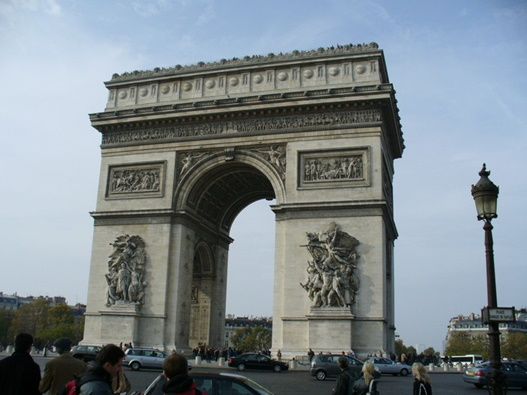
\includegraphics[scale=0.5]{images/obr1.jpg}
\caption{Vítězný oblouk 1}
\label{oblouk}

\end{figure}

V roce 1840 byl mrtvý císař přenesen během pohřebních slavností branou oblouku do Invalidovny, v roce 1885 zde byla na jednu noc vystavena rakev se zesnulým velký francouzským básníkem Victorem Hugem a 26. srpna 1944 zde oslavil francouzský národ v čele s generálem de Gaullem\index{Gaullem} osvobození.\\
\\
Pod Vítězným obloukem se nachází Památník Neznámého vojáka (Le soldat inconnu), který zde byl slavnostně pohřben 11. listopadu 1920. Oblouk od té doby slouží také jako národní pomník všech Francouzů padlých v mnoha válkách. Vyhlídková terasa skýtá velkolepý pohled na osu Louvre – Náměstí svornosti (Place de la Concorde) – La défence. Dějiny památníku dokumentuje malé Muzeum Vítězného oblouku – Musée de l'Arc de Triomphe.\cite{lacko}\\
\begin{figure}[h!]
\centering
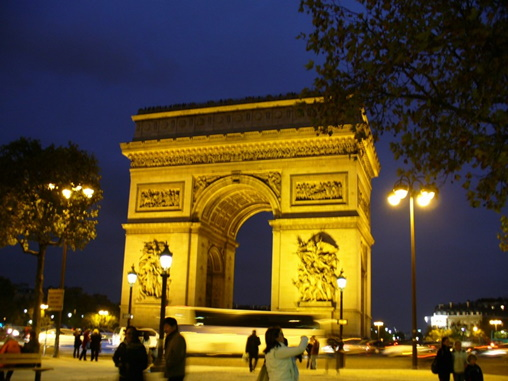
\includegraphics[scale=0.5]{images/obr2.jpg}
\caption{Vítězný oblouk 2}
\label{oblouk1}
\end{figure}
\\
Při pohledu na oblouk ze Champs-Elysées spatříte v levé spodní části reliéf zvaný Napoleonův triumf. Oslavuje vídeňskou smlouvu podepsanou v roce 1810, kdy Napoleonova říše prožívala vrcholný rozkvět. Nad Napoleonovým triumfem je umístěn reliéf líčící vítězství Napoleona nad Turky v roce 1799. Stejnou událost připomíná plátno francouzského malíře Antoina Grosa\index{Grosa}, vystavené v paláci ve Versailles. Další vítězství v bitvě je vyobrazeno na vlysu na severní straně oblouku. Přibližuje početně slabé Napoleonovo vojsko rozbíjející led na moravském rybníku. Utonuly tak tisíce nepřátelských vojáků a Francouzi zvítězili. Jeden z nejpůsobivějších reliéfů spatříte na přední části oblouku vpravo dole. Zachycuje francouzské občany odcházející bránit svůj národ před Rakušany a Prusy. Pohřeb generála Marceaua, který padl v bitvě proti rakouské armádě v roce 1796, kterou porazil pouhý rok předtím, je zvěčněn na vlysu nad reliéfem Odchodu dobrovolníků. Východní strana vlysu znázorňuje odchod francouzských vojsk o bitvy a západní jejich vítězný návrat.


\section{Eiffelova věž (Tour Eiffel)}
Asi nejznámějším monumentem Paříže vůbec je 324 metrů vysoká Eiffelova věž (obrázek ~\ref{vez1} a ~\ref{vez2}) Eiffelova postavená ze železa, přezdívaná „Železná dáma“ (La Dame de Fer). Nachází se na Champ de Mars na levém břehu řeky Seiny. Eiffelovu věž navštíví ročně přes 6 milionů návštěvníků.
\\
\begin{figure}[h!]
\centering
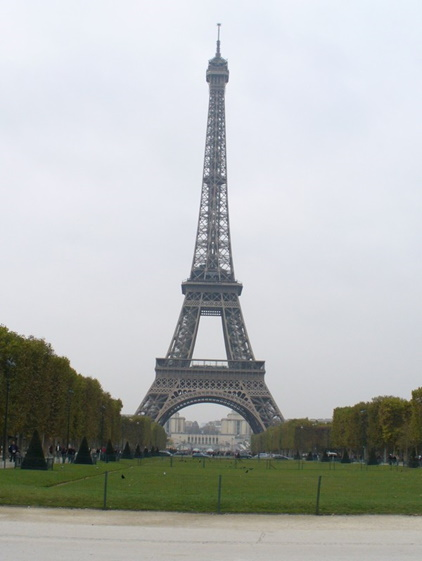
\includegraphics[scale=0.5]{images/obr3E.jpg}
\caption{Eiffelova věž}
\label{vez1}
\end{figure}
\\
\subsubsection{Kudy nahoru}
Věž je třípatrová, nahoru se dá dostat pěšky po schodech i výtahem. Schody vedou jen do druhého patra, výtahy z přízemí také do prvního a druhého patra, do třetího patra jede zase jiný výtah. Výtahy jsou celkem tři – ve východním, severním a západním pilíři.\\\\První plošina (57 m)\\
\\
Poskytuje audiovizuální muzeum ukazující stavbu a panoramatický výhled na Paříž, jsou zde restaurace.\\
\\
Druhá plošina (115 m)\\
\\
Jsou zde restaurace. Často je odtud lepší výhled než z vrcholu věže.\\
Třetí plošina (274 m)\\
\\
Dostupná jen výtahem. Je zde bar. Při dobré viditelnosti je odtud vidět i katedrála v Chartres, až na vzdálenost 65 km.\\
\\
Kromě Eiffelovy věže je krásný pohled na Paříž také od Sacré Coeur na kopci Montmartre. Pokud vás zajímá nejen pohled na Paříž, ale také na Eiffelovu věž, nejlepší pohled je od Pallais de Chaillot.
\\

\subsubsection{Historie Eiffelovy věže}
Eiffelova věž byla navržena architektem Gustavem Eiffelem (mj. autorem Sochy svobody) na počest 100. výročí Velké francouzské revoluce a Světové výstavy v roce 1889. V době vzniku byla nejvyšší stavbou světa. Původně byla věž postavena pouze na období 20 let. Mezitím získala ale svůj význam jako meteorologická stanice, proto zůstala zachována. Později se stala věž také centrem letového provozu a rozhlasového a televizního vysílání.\\
\\
Původně se věž pařížanům nelíbila, byla považována za ošklivé mostrum, architekti, spisovatelé a další umělci (Maupassant, Dumas ml., Gounod) se spojili v akci „300“ za odstranění monstra. Roku 1909 měla být věž zbourána z důvodu prošlé koncese. Počátkem 20. století se ale začala objevovat na obrazech (Pissaro, Utrillo, Seurat, Delaunay) a začali ji oslavovat i básníci (Cocteau, Apollinaire).\\\\V roce 1923 byla Antoinem Bourdellem pod Eiffelovu věž umístěna busta Eiffela, jako ocenění za jeho práci.\\

\subsubsection{Praktické informace}
\begin{itemize}
    \item Kudy na Eiffelovku: stanice metra 6 -- Passy.
    \item Vstupné: pěšky (1. a 2. patro) 3,80 €, výtah 1. patro 4,20 €, výtah 2. patro 7,70 €, výtah 3. patro 11,00 €.
    \item Nejlepší výhled: hodinu před západem slunce je nejlepší světlo.
\end{itemize}
\begin{figure}[h!]
\centering
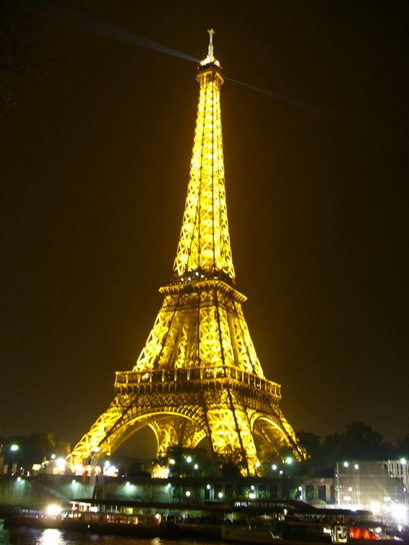
\includegraphics[scale=0.5]{images/obr4E.jpg}
\caption{Osvětlená Eiffelova věž}
\label{vez2}

\end{figure}

